%! Author = Vojta
%! Date = 21.1.2024

\chapter{Návrh}

\section{Úvod}
Návrh je důležitým krokem v procesu vývoje, který předchází samotné implementaci a testování. V této kapitole bude podrobně rozebrán postup a myšlenkové procesy, které vedou k vytvoření sbírky komponent přívětivé jak pro uživatele, tak pro vývojáře. Nejprve bude popsán vývoj a struktura dokumentace, která je nezbytná pro správné použití a rozšíření UI kolekce, dále návrh samotných komponent a příprava Figma kitu, který slouží jako most mezi designéry a vývojáři. Také bude vysvětlen význam a využití bloků, které umožňují rychlejší a efektivnější vývoj webových aplikací. Nakonec bude popsán návrh CLI, které umožňuje snadné přidávání komponent do existujících projektů.

\clearpage

\section{Dokumentace}
Součástí každého softwarového projektu by měla být kvalitní dokumentace (ačkoliv se tak často neděje). Pro účely této sbírky znovupoužitelných UI komponent je potřeba připravit dokumentaci, která nejen vysvětluje jak používat jednotlivé komponenty, ale také poskytuje ucelený pohled na architekturu a filozofii za celým projektem. Tato sekce se zabývá obsahem dokumentace a její strukturou.

\subsection{Obsah dokumentace}
Hlavním cílem dokumentace je poskytnout vývojářům všechny potřebné informace.

\begin{description}
  \item[Úvod do principů a filozofie knihovny] Vysvětlení, v čem se knihovna liší od typických UI knihoven.
  \item[Návod k použití] Průvodce krok za krokem, jak začít využívat komponenty knihovny.
  \item[Podpůrné materiály] Doprovodné zdroje, například Figma kit a tipy pro řešení problémů.
  \item[Přehled komponent] Detailní popis každé komponenty, včetně jejího účelu, možností konfigurace a příkladů použití.
\end{description}

Dokumentace bude rozdělena do dvou hlavních sekcí: \emph{Getting Started} a \emph{Components}. Sekce \emph{Getting Started} bude poskytovat uživatelům všechny základní informace potřebné pro rychlý start s knihovnou, včetně instalace, konfigurace a prvních kroků s komponentami. To pomůže novým uživatelům snadno se orientovat v možnostech knihovny a začít s jejím používáním. Sekce \emph{Components} se bude zabývat detailním popisem jednotlivých komponent, včetně jejich vlastností, možností přizpůsobení a příkladů použití.

\subsection{Dokumentace konkrétních komponent}
Stránka dokumentace pro každou konkrétní komponentu bude jasně strukturovaná a bude poskytovat ucelené informace, které usnadní její použití. Na začátku stránky bude uveden název komponenty a pod ním krátký popis, který objasňuje, k čemu komponenta slouží. Bude následovat sekce s ukázkou komponenty, doplněná o příslušný zdrojový kód, který bude ilustrovat, jak lze komponentu použít. Návod k instalaci bude popisovat, jak komponentu přidat do projektu, ať už pomocí CLI nástroje nebo prostřednictvím manuálního kopírování kódu. Na stránce vývojáři naleznou také seznam \emph{props} a \emph{slotů}, které umožňují přizpůsobit komponentu specifickým potřebám. Stránka může dále obsahovat další poznámky a varování ohledně specifik komponenty, jako jsou potenciální chyby, omezení, nebo doporučené postupy.

\section{Figma Kit}
Figma Kit bude vyvinut s cílem poskytnout designérům a vývojářům snadno použitelnou sadu komponent, které jim umožní efektivně navrhovat a prototypovat aplikace. Kit bude obsahovat komponenty UI kolekce, přesně tak, jak jsou definovány ve finální implementaci, což zajišťuje, že designy jsou plně kompatibilní s konečnou implementací. Připravené budou komponenty jako tlačítka, inputy, plovoucí prvky a mnoho dalšího, což designérům umožňuje sestavit uživatelské rozhraní rychle a s vysokou mírou přesnosti.

Pro vývojáře pak bude snadné převést designy vytvořené v Figmě do kódu, protože mohou snadno identifikovat, které komponenty mají být použity. Díky definovaným proměnným lze snadno přizpůsobit barvy, velikosti a další vlastnosti komponent, které vývojáři mohou specifikovat v rámci projektu.

U každé komponenty se bude nacházet odkaz do dokumentace, kde mohou jak designéři, tak vývojáři najít podrobné informace o tom, k čemu komponenta je a jaké jsou její možnosti.

\begin{figure}[H]
  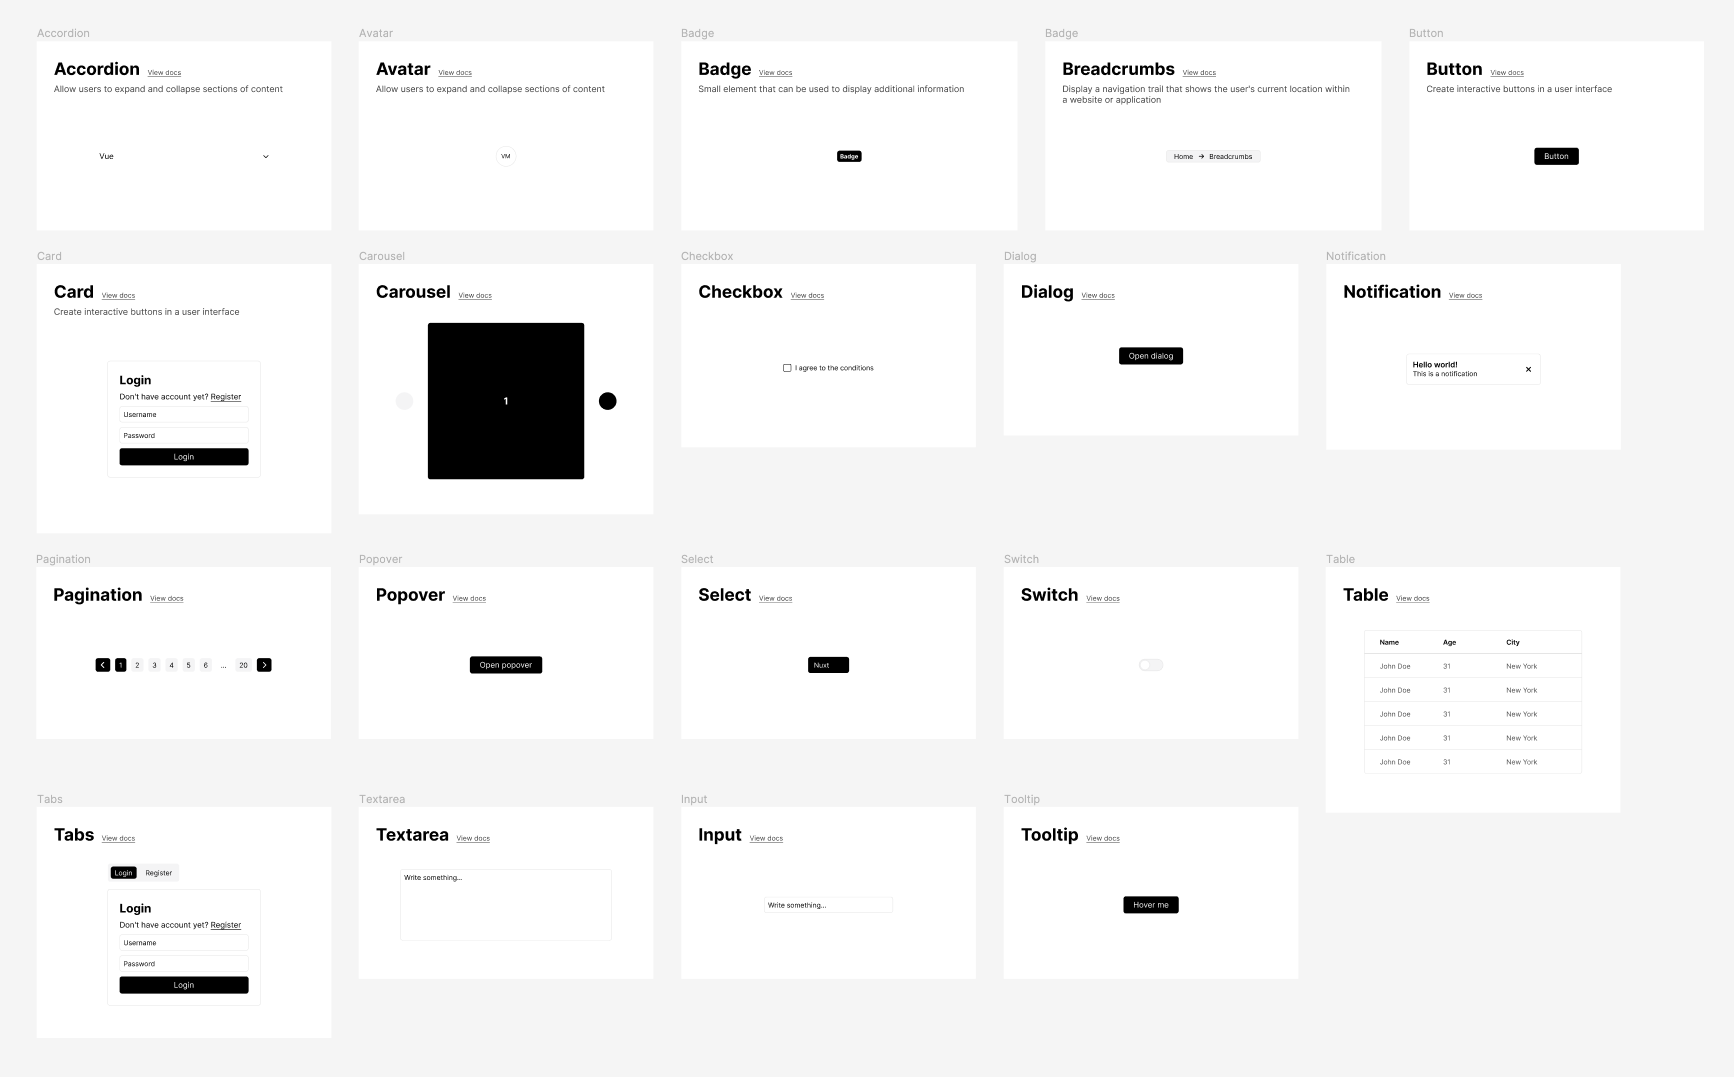
\includegraphics[width=\textwidth]{images/figma-kit}
  \caption{Komponenty ve Figmě} \label{picture:figma-kit}
\end{figure}

\clearpage

\section{Komponenty}
Výběr těchto komponent je založen na jejich základní funkčnosti a častém využití ve webových aplikacích. Každá z těchto komponent přináší konkrétní užitečné vlastnosti, které zlepšují uživatelský zážitek a zjednodušují vývojový proces. Tento soubor základních komponent vytváří pevný základ pro další rozšiřování sbírky. V budoucnu bude sbírka doplněna o další komponenty, které budou reagovat na specifické potřeby a požadavky vývojářů.

\subsection{Accordion}
\emph{Accordion} je komponenta určená k zobrazení a skrytí obsahu v rozbalovacích sekcích. Umožňuje uživatelům zobrazit pouze relevantní část informací a zbytek skrýt, čímž šetří místo na obrazovce a zvyšuje přehlednost. \emph{Accordion} se často používá pro často kladené otázky (FAQ) nebo detaily produktů.

\begin{figure}[H]
  \centering
  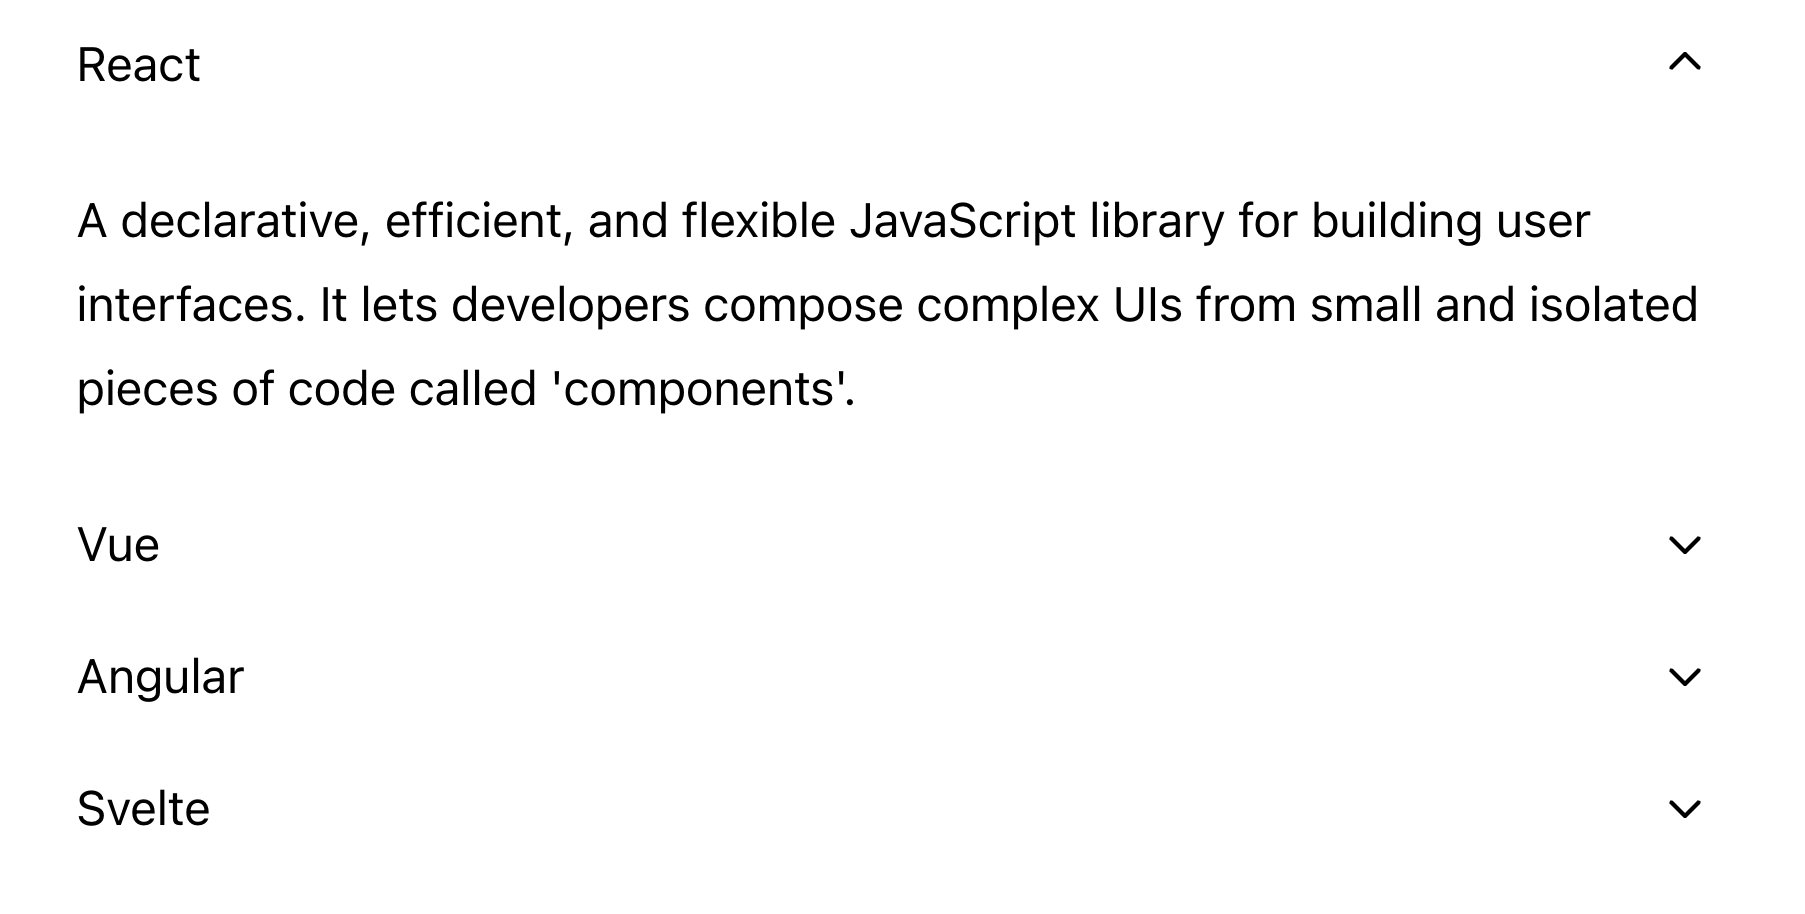
\includegraphics[width=10cm]{images/accordion}
  \captionsetup{justification=centering,margin=2cm}
  \caption{Accordion} \label{picture:accordion}
\end{figure}

\subsection{Avatar}
Avatar je vizuální reprezentace uživatele, obvykle v podobě kruhového nebo čtvercového obrázku. Používá se k identifikaci uživatelů v aplikacích, například v uživatelských profilech, seznamu kontaktů nebo diskuzních fórech. Avatar může obsahovat iniciály uživatele, ikonu nebo fotografii.

\begin{figure}[H]
  \centering
  
\includegraphics[width=2cm]{images/avatar}
  \captionsetup{justification=centering,margin=2cm}
  \caption{Avatar} \label{picture:avatar}
\end{figure}

\subsection{Badge}
\emph{Badge} je komponenta používaná k zobrazení malého označení nebo indikátoru, který poskytuje dodatečnou informaci. Typickým použitím je například zobrazení štítků, počtu nepřečtených zpráv, oznámení nebo označení nových funkcí v aplikaci.

\begin{figure}[H]
  \centering
  
\includegraphics[width=2cm]{images/badge}
  \captionsetup{justification=centering,margin=2cm}
  \caption{Badge} \label{picture:badge}
\end{figure}

\subsection{Breadcrumbs}
Breadcrumbs slouží k navigaci a orientaci uživatelů na webových stránkách nebo v aplikacích. Zobrazuje hierarchii stránek, což uživatelům umožňuje rychle se vrátit na předchozí úrovně nebo domovskou stránku. Breadcrumbs zlepšují uživatelskou zkušenost tím, že usnadňují navigaci v komplexních strukturách.

\begin{figure}[H]
  \centering
  
\includegraphics[width=5cm]{images/breadcrumbs}
  \captionsetup{justification=centering,margin=2cm}
  \caption{Breadcrumbs} \label{picture:breadcrumbs}
\end{figure}

\subsection{Button}
\emph{Button} je základní interaktivní komponenta, která umožňuje uživatelům provádět akce, jako je odeslání formuláře, zahájení procesu nebo navigace na jinou stránku. \emph{Buttony} mohou mít různé styly a velikosti, aby odpovídaly specifickým požadavkům aplikace nebo designu.

\begin{figure}[H]
  \centering
  
\includegraphics[width=3cm]{images/button}
  \captionsetup{justification=centering,margin=2cm}
  \caption{Button} \label{picture:button}
\end{figure}

\subsection{Card}
\emph{Card} je vizuální komponenta, která obklopuje obsah a poskytuje kontext. Karty jsou často používány k organizaci informací do samostatných bloků, které mohou obsahovat obrázky, texty a akční tlačítka. \emph{Cards} se využívají v \emph{dashboardech}, produktech nebo profilech uživatelů.

\begin{figure}[H]
  \centering
  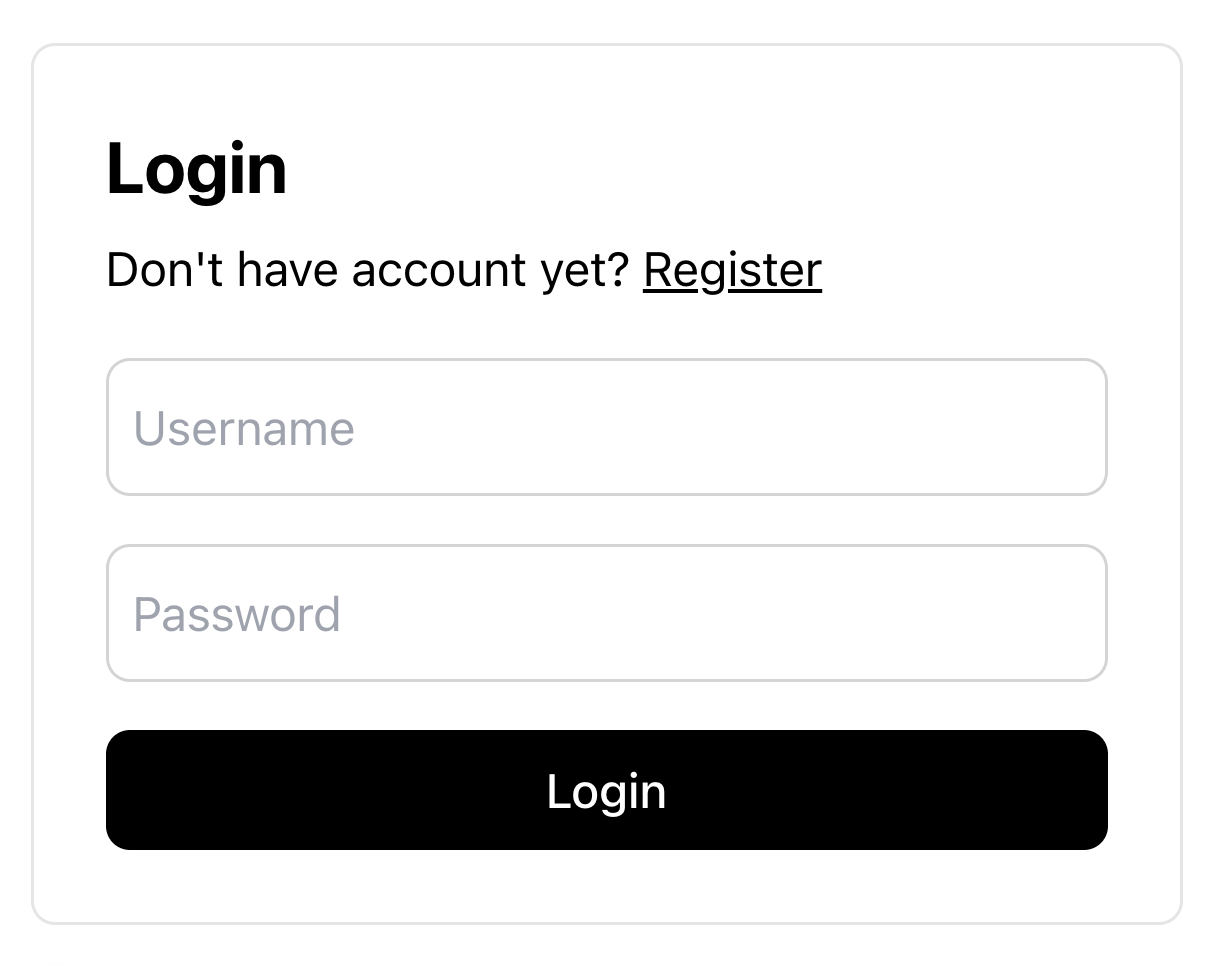
\includegraphics[width=7cm]{images/card}
  \captionsetup{justification=centering,margin=2cm}
  \caption{Card} \label{picture:card}
\end{figure}

\subsection{Carousel}
\emph{Carousel} je komponenta umožňující zobrazení více položek (obrázků, karet) v rotující nebo posuvné formě. Umožňuje efektivně využít prostor a zobrazit více obsahu na omezené ploše, což je ideální pro prezentaci galerií, doporučených produktů nebo novinek.

\begin{figure}[H]
  \centering
  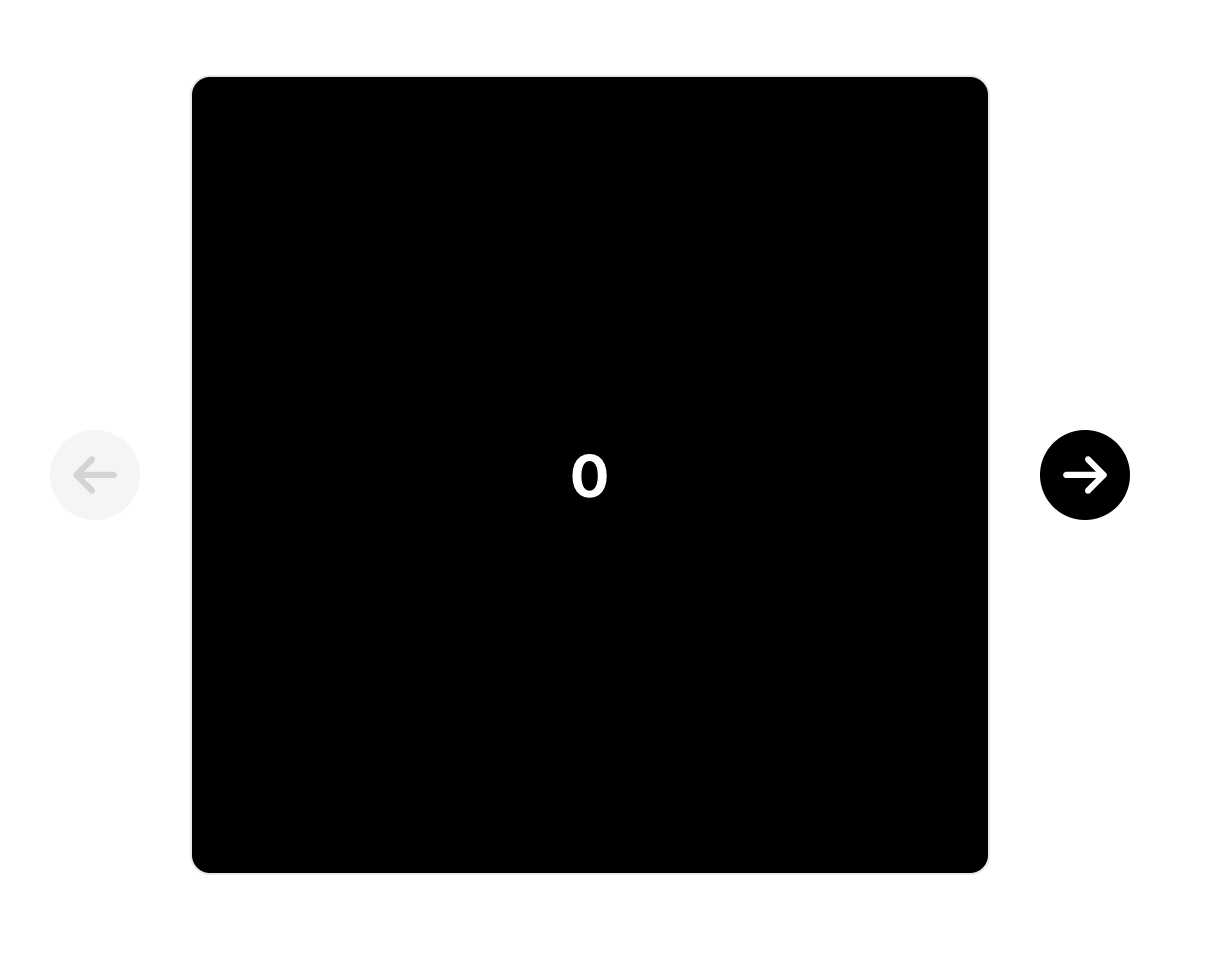
\includegraphics[width=7cm]{images/carousel}
  \captionsetup{justification=centering,margin=2cm}
  \caption{Carousel} \label{picture:carousel}
\end{figure}

\subsection{Checkbox}
\emph{Checkbox} je vstupní komponenta, která umožňuje uživatelům vybrat jednu nebo více možností z nabídky. Používá se ve formulářích, nastaveních a dalších interaktivních prvcích, kde je potřeba více výběrů.

\begin{figure}[H]
  \centering
  
\includegraphics[width=5cm]{images/checkbox}
  \captionsetup{justification=centering,margin=2cm}
  \caption{Checkbox} \label{picture:checkbox}
\end{figure}

\subsection{Dialog}
Dialog je modální okno, které se objevuje nad hlavním obsahem stránky, aby poskytlo důležité informace nebo vyžádalo potvrzení akce od uživatele. Dialogy jsou používány pro potvrzovací zprávy, formuláře nebo upozornění, která vyžadují okamžitou pozornost uživatele.

\subsection{Icon}
\emph{Icon} je grafický symbol reprezentující akci, objekt nebo koncept. Ikony se používají ke zlepšení vizuální komunikace v uživatelských rozhraních, často jako doplněk textových popisků. Mohou být použity v tlačítkách, navigačních lištách nebo jako vizuální indikátory.

\subsection{Loading}
\emph{Loading} je komponenta, která indikuje probíhající proces nebo načítání obsahu. Pomáhá uživatelům pochopit, že akce je v procesu a vyžaduje čas. \emph{Loading} indikátory mohou mít různé formy, například točící se kolečko, prodlužující se pruh nebo blikající tečky.

\begin{figure}[H]
  \centering
  \subfloat{
\includegraphics[width=2cm]{images/loading-circle}}
  \hspace{1cm}
  \subfloat{
\includegraphics[width=3cm]{images/loading-dots}}\\
  \subfloat{
\includegraphics[width=10cm]{images/loading-progress}}
  \captionsetup{justification=centering,margin=2cm}
  \caption{Loading}
\end{figure}

\subsection{Notification}
\emph{Notification} je komponenta pro zobrazení krátkých zpráv nebo upozornění uživatelům. Může informovat o úspěšných akcích, varováních, chybách nebo nových událostech. Notifikace mohou být dočasné nebo trvalé, a obvykle se zobrazují v rohu obrazovky.

\begin{figure}[H]
  \centering
  
\includegraphics[width=7cm]{images/notification}
  \captionsetup{justification=centering,margin=2cm}
  \caption{Notification} \label{picture:notification}
\end{figure}

\subsection{Pagination}
\emph{Pagination} je komponenta, která rozděluje obsah do více stránek a poskytuje ovládací prvky pro navigaci mezi nimi. Používá se v aplikacích a na webových stránkách s velkým množstvím dat, aby se usnadnila jejich přehlednost a navigace.

\begin{figure}[H]
  \centering
  
\includegraphics[width=7cm]{images/pagination}
  \captionsetup{justification=centering,margin=2cm}
  \caption{Pagination} \label{picture:pagination}
\end{figure}

\subsection{Popover}
\emph{Popover} je komponenta, která zobrazuje dodatečný obsah v malém okně, které se objevuje pod obsahem po interakci uživatele. \emph{Popover} se často používá pro kontextové nabídky, tipy nebo formuláře, které vyžadují uživatelovu pozornost, aniž by opustil aktuální stránku.

\begin{figure}[H]
  \centering
  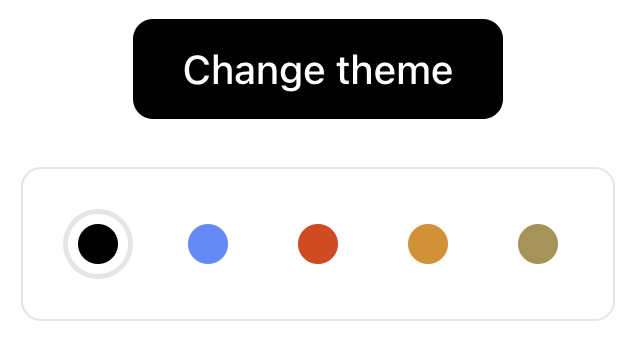
\includegraphics[width=5cm]{images/popover}
  \captionsetup{justification=centering,margin=2cm}
  \caption{Popover} \label{picture:popover}
\end{figure}

\subsection{Select}
\emph{Select} je vstupní komponenta umožňující uživatelům vybrat jednu možnost z rozbalovací nabídky. Používá se ve formulářích a nastaveních, kde je potřeba vybrat z předdefinovaného seznamu hodnot. \emph{Select} komponenty mohou být jednoduché nebo víceúrovňové.

\begin{figure}[H]
  \centering
  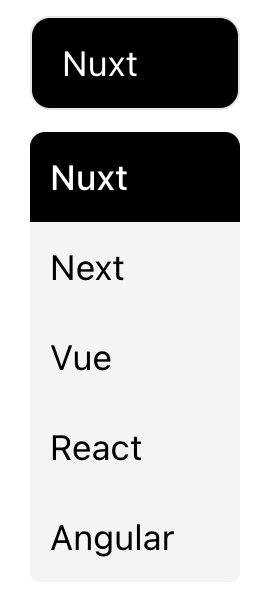
\includegraphics[width=3cm]{images/select}
  \captionsetup{justification=centering,margin=2cm}
  \caption{Select} \label{picture:select}
\end{figure}

\subsection{Sidebar}
\emph{Sidebar} je vertikální panel, který poskytuje navigaci nebo další obsah vedle hlavního obsahu stránky. Sidebary se používají pro menu, seznamy položek nebo další interaktivní prvky, které zůstávají přístupné během procházení hlavního obsahu.

\subsection{Switch}
\emph{Switch} je komponenta, která umožňuje uživatelům přepínat mezi dvěma stavy, obvykle zapnuto a vypnuto. Používá se pro nastavení, která mají binární volbu, jako je povolení nebo zakázání funkcí.

\begin{figure}[H]
  \centering
  \subfloat{
\includegraphics[width=2cm]{images/switch}\label{picture:documentation:switch}}
  \hspace{1cm}
  \subfloat{
\includegraphics[width=2cm]{images/switch-on}\label{picture:documentation:switch-on}}
  \captionsetup{justification=centering,margin=2cm}
  \caption{Switch}
\end{figure}

\subsection{Table}
\emph{Table} je komponenta pro zobrazení strukturovaných dat ve formě tabulky. Tabulky se používají k organizaci informací do řádků a sloupců, což umožňuje snadné srovnání a analýzu dat. Jsou běžně používány v dashboardech, reportech a dalších datově orientovaných aplikacích.

\begin{figure}[H]
  \centering
  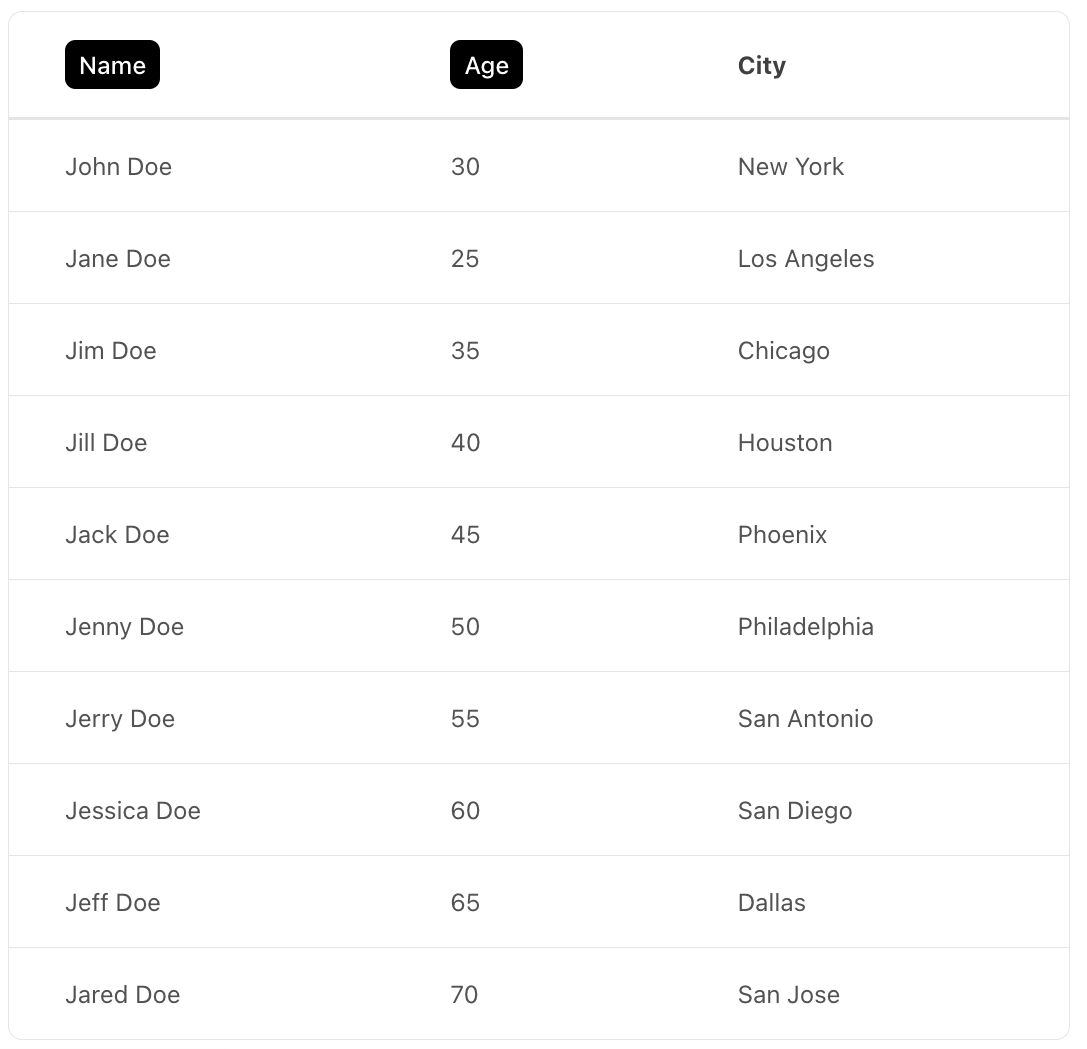
\includegraphics[width=10cm]{images/table}
  \captionsetup{justification=centering,margin=2cm}
  \caption{Table} \label{picture:table}
\end{figure}

\clearpage

\subsection{Tabs}
\emph{Tabs} jsou komponenty, které umožňují uživatelům přepínat mezi různými částmi obsahu na jedné stránce. \emph{Tabs} zlepšují organizaci a přehlednost, když je potřeba prezentovat velké množství informací v omezeném prostoru. Každá karta obsahuje jiný obsah, který se zobrazí po kliknutí na záložku.

\begin{figure}[H]
  \centering
  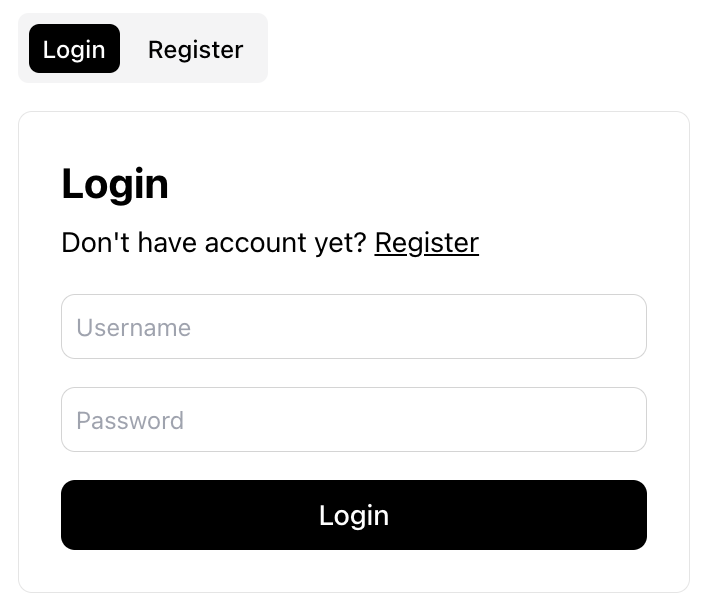
\includegraphics[width=7cm]{images/tabs}
  \captionsetup{justification=centering,margin=2cm}
  \caption{Tabs} \label{picture:tabs}
\end{figure}

\subsection{Textarea}
\emph{Textarea} je vstupní komponenta, která umožňuje uživatelům zadat víceřádkový text. Používá se ve formulářích, kde je potřeba více místa pro text, například v komentářích, poznámkách nebo popisech.

\begin{figure}[H]
  \centering
  
\includegraphics[width=10cm]{images/textarea}
  \captionsetup{justification=centering,margin=2cm}
  \caption{Textarea} \label{picture:textarea}
\end{figure}

\subsection{Text input}
\emph{Text input} je základní vstupní pole, které umožňuje uživatelům zadávat text. Používá se ve formulářích pro zadání jednoduchých textových informací, jako jsou jména, e-maily nebo hesla. \emph{Text input} může mít různé typy, například text, email, password nebo number.

\begin{figure}[H]
  \centering
  
\includegraphics[width=10cm]{images/textinput}
  \captionsetup{justification=centering,margin=2cm}
  \caption{Textinput} \label{picture:textinput}
\end{figure}

\subsection{Tooltip}
\emph{Tooltip} je komponenta, která poskytuje dodatečné informace o prvku, když na něj uživatel najede myší nebo se na něj jiným způsobem zaměří. \emph{Tooltipy} se používají ke zlepšení uživatelského zážitku tím, že poskytují kontext nebo vysvětlení bez nutnosti zabírat místo na obrazovce.

\begin{figure}[H]
  \centering
  
\includegraphics[width=3cm]{images/tooltip}
  \captionsetup{justification=centering,margin=2cm}
  \caption{Tooltip} \label{picture:tooltip}
\end{figure}

\clearpage

\section{Bloky}
Bloky jsou větší, komplexní komponenty, které fungují jako samostatné sekce webových aplikací. Dělí se na dva typy a to sice pro jedno použití a znovupoužitelné. Mezi komponenty pro jedno použití patří např. úvodní stránka. Tyto bloky většinou obsahují statický obsah, který se nemění a je na vývojářích, aby textace a obsah doplnili dle potřeby. Naopak znovupoužitelné bloky jsou komponenty, které se mohou použít na více místech aplikace. Mezi ně patří např. sekce, které se mohou nacházet na jedné stránce několikrát. \footnote{Tento nápad byl přidán během tvorby této práce i do knihovny shadcn/ui. Vzhledem k přidání do této úspěšné knihovny se potrzuje, že tato myšlenka je správná a má smysl.}

Bloky značně zlepšují efektivitu vývoje tím, že standardizují často používané UI prvky do předdefinovaných šablon. Díky tomu mohou vývojáři snadno implementovat a opakovaně používat komplexní UI struktury bez nutnosti opětovného kódování nebo redesignu těchto částí pro každý nový projekt.

Hlavní přínosy bloků spočívají v jejich schopnosti snižovat redundantní kód a zvyšovat znovupoužitelnost komponent napříč projekty. Díky konzistentní implementaci jednotlivých bloků mohou vývojáři efektivně reagovat na nové požadavky nebo změny v designu bez rozsáhlých úprav celé aplikace.

\begin{figure}[H]
  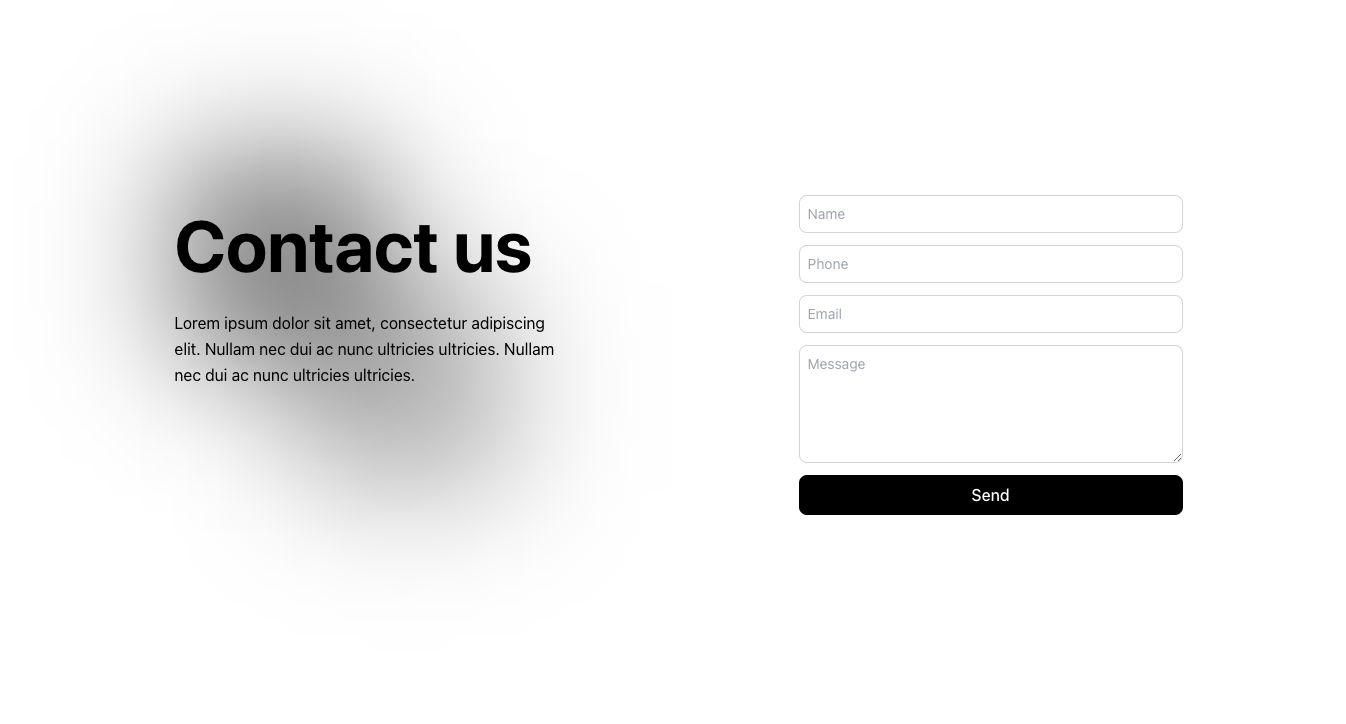
\includegraphics[width=\textwidth]{images/block-contact}
  \caption{Blok s kontaktním formulářem} \label{picture:block-contact}
\end{figure}

\subsection{Hero}

\emph{Hero sekce} je úvodní část stránky, která zaujme návštěvníky a poskytuje hlavní informace nebo klíčové sdělení. Obvykle se nachází v horní části stránky a obsahuje poutavý obrázek nebo video, výrazný nadpis a krátký popis. Je navržena tak, aby upoutala pozornost uživatelů a povzbudila je k dalšímu prozkoumání webu nebo provedení určité akce, například kliknutí na tlačítko s výzvou k akci (CTA).

\subsection{Section}

\emph{Section} je univerzální blok, který rozděluje obsah stránky do logických částí. Každá sekce může mít vlastní obsah, jako jsou texty, obrázky nebo interaktivní prvky, a slouží k organizaci informací na stránce tak, aby byly přehledné a snadno čitelné. Sekce pomáhají strukturovat stránku a usnadňují uživatelům orientaci a nalezení relevantních informací.

\subsection{Features}

\emph{Features} blok slouží k prezentaci hlavních funkcí nebo výhod produktu či služby. Obvykle se skládá z řady ikon nebo obrázků doplněných krátkými popisy, které stručně a jasně vysvětlují, co produkt nebo služba nabízí. Tento blok pomáhá uživatelům rychle pochopit, jaké benefity mohou očekávat, a usnadňuje rozhodování o koupi nebo dalším využití.

\subsection{References}

\emph{References} blok je určen k zobrazení referencí, recenzí nebo citací od spokojených zákazníků či partnerů. Tento blok zvyšuje důvěryhodnost a kredibilitu produktu nebo služby tím, že poskytuje sociální důkazy o jeho kvalitě a spolehlivosti. Obsahuje často fotografie, jména a krátké výpovědi od skutečných uživatelů, což pomáhá budovat důvěru u potenciálních zákazníků.

\subsection{Contact}

\emph{Contact} blok slouží k zobrazení kontaktních informací a formulářů, které umožňují uživatelům snadno se spojit s provozovatelem webu nebo podpůrným týmem. Tento blok obvykle obsahuje informace jako jméno, telefonní číslo a e-mailová adresa. Může také obsahovat kontaktní formulář, který uživatelům umožňuje rychle zaslat zprávu nebo dotaz přímo z webové stránky.

\subsection{Auth}

\emph{Auth} blok se používá pro autentizaci uživatelů, tedy pro přihlášení, registraci nebo obnovení hesla. Obsahuje formuláře, které uživatelům umožňují zadávat své přihlašovací údaje, vytvářet nové účty nebo obnovit zapomenuté heslo. Tento blok je navržen pro webové aplikace, které vyžadují bezpečný přístup k uživatelským účtům a osobním informacím.

\subsection{Blog}

Blog blok slouží k zobrazení seznamu článků nebo příspěvků na blogu. Tento blok obvykle obsahuje náhledy článků s titulky, krátkými úryvky a odkazy na celé články. Blog sekce pomáhá udržovat web aktuální a informativní, zlepšuje SEO a poskytuje uživatelům hodnotný obsah, který je může zaujmout a přivést zpět na web.

\subsection{Header}

\emph{Header} je horní část webové stránky, která obvykle obsahuje logo, navigační menu a další prvky, jako jsou odkazy na přihlášení, nákupní košík nebo vyhledávací pole. \emph{Header} je důležitým prvkem každé webové stránky, protože poskytuje uživatelům rychlý přístup k hlavním sekcím webu a usnadňuje navigaci. Důraz na jednoduchost a přehlednost v \emph{headeru} zlepšuje uživatelskou zkušenost a orientaci.

\section{CLI}
Vzhledem k tomu, že se nejedná o klasickou knihovnu s principem balíčkování, není možné využít package manažerů pro instalaci. Nabízí se tedy dvě možnosti.

\begin{enumerate}
  \item Manuální kopírování souborů do projektu.
  \item Použití CLI, které bude zajišťovat inicializaci a přidávání komponent do projektů.
\end{enumerate}

Manuální kopírování souborů do projektu je sice možné, ale zdlouhavé a náchylné k chybám. Na druhou stranu je tato možnost velmi jednoduchá a nevyžaduje žádné další kroky. Ideální je tedy kombinace obou možností.
Pokud vývojář z nějakých důvodů nebude chtít použít CLI, může si soubory zkopírovat z Githubu a ručně je přidat do projektu. Odkazy na Github budou dostupné v dokumentaci.

Pro usnadnění práce s UI knihovnou je tedy potřeba vyvinout CLI, které pomůže s inicializací a přidáváním komponent do projektů.

\subsection{Inicializace}
Inicializace knihovny prostřednictvím CLI zajišťuje, že jsou přidány všechny závislosti a další potřebné soubory jsou připraveny k použití ihned po vytvoření nového projektu. Příkaz pro inicializaci může vypadat například takto \mintinline{console}|npx @v-moravec/ui init|. V rámci tohoto příkazu je potřeba zkontrolovat, zda již soubory neexistují. Pokud by existovaly, měl by uživatel dostat možnost zvolit, zda chce přepsat stávající soubory nebo pokračovat bez změn. V případě chybějících souborů se automaticky vytvoří nové.

Získání souborů a závislostí by mělo být automatizováno, aby se zabránilo chybám a zjednodušil se vývoj knihovny. Nejjednodušší způsob je soubory zpřístupnit v rámci API části dokumentace (webové aplikace), odkud je možné s nimi pracovat na úrovní CLI. Jak toto funguje, bude popsáno v kapitole \ref{ch:implementation}. Pro tuto automatizaci je možné využít vlastních Nuxt modulů. Jako inspiraci lze použít modul, který využívá knihovna Nuxt UI. \cite{NuxtUISourceCodeModule}

\subsection{Přidání komponent}
Přidání komponent a bloků využije stejného principu jako inicializace projektu. Příkaz pro přidání komponenty může vypadat například takto:\\

\mintinline{console}|npx @v-moravec/ui add [...componentName/blockName]|\\

Při přidání komponenty je potřeba zkontrolovat, zda již soubory neexistují. Pokud by existovaly, měl by uživatel dostat možnost zvolit, zda chce přepsat stávající soubory nebo pokračovat bez změn. V případě chybějících souborů se automaticky vytvoří nové.

Z hlediska zdrojového kódu komponent a bloků bude potřeba více modulů, které na API vystaví všechny potřebné informace. Také bude potřeba v rámci každého souboru zjistit jeho závislosti a to na externích knihovnách, komponentách v rámci knihovny a dalších souborech, jako například composables. Toho je možné dosáhnout pomocí \emph{pattern matchingu}.

\subsection{Publikace balíčku}
Jak bylo popsáno v sekci o technologiích, pro správu verzí balíčku se používá nástroj Changesets. Workflow pak bude vypadat následovně:

\begin{enumerate}
  \item Vytvoření změn v kódu.
  \item Vytvoření nové verze pomocí Changeset.
  \item Nahrání změn na GitHub.
  \item Spuštění GitHub Actions workflow pro publikaci balíčku.
  \item Publikace nové verze balíčku.
\end{enumerate}

Díky této automatizaci bude možné rychle a bezpečně publikovat nové verze balíčku, aniž by bylo nutné manuálně upravovat potřebné soubory.

\section{Závěr}
V této kapitole byly popsány kroky a procesy vedoucí k navržení sbírky znovupoužitelných Nuxt komponent. Byly identifikovány a zdokumentovány prvky, které ovlivňují design a implementaci UI komponent.

Hlavním cílem navrhované sbírky komponent je vytvoření robustního základu, který umožní efektivní vývoj webových aplikací s využitím moderních frontend technologií. Tento návrh reflektuje nejnovější trendy ve vývoji webových aplikací, a také přináší řadu nástrojů, které podporují celý životní cyklus vývoje od návrhu po nasazení a údržbu.

V další kapitole Implementace se práce zaměří na vytvoření navržených komponent. Diskutovány budou také výzvy a řešení, která byla během implementace identifikována.


